% !TeX root = ../libro.tex
% !TeX encoding = utf8
\chapter{Aplicación: Calentamiento y enfriamiento de edificios}
Como aplicación sobre lo estudiado anteriormente, vamos a formular un modelo matemático que describa la temperatura dentro de un edificio, como función de la temperatura exterior, el calor generado dentro del edificio y el calefactor o el aire acondicionado.

Un enfoque natural para modelar la temperatura dentro de un edificio es el uso del análisis por compartimentos.
\section{Edificio como habitación única}
Sea $T(t)$ la temperatura dentro del edificio en el instante $t$ y veamos al edificio como un único compartimento, es decir, sin estar dividido en varias habitaciones. Entonces la razón de cambio en la temperatura queda determinada por todos los factores que generan o disipan calor. Tomaremos en cuenta tres factores principales que afectan la temperatura dentro del edificio:
\begin{itemize}
	\item En primer lugar está el calor generado por las personas, las luces y las máquinas dentro del edificio. Esto causa una razón de incremento en la temperatura que denotaremos por $H(t)$.
	\item En segundo lugar está el calentamiento (o enfriamiento) proporcionado por la calefacción (o el aire acondicionado).  Esta razón de incremento (o decremento) en temperatura será representada por $U(t)$.
	\item El tercer factor es el efecto de la temperatura exterior $M(t)$ sobre la temperatura dentro del edificio. La evidencia experimental ha mostrado que este factor se puede modelar mediante la \textbf{ley de enfriamiento de Newton}.
	
	Esta ley establece que hay una razón de cambio de la temperatura $T(t)$ que es proporcional a la diferencia entre la temperatura exterior $M(t)$ y la temperatura interior $T(t)$. Es decir, la razón de cambio en temperatura del edificio debida a $M(t)$ es 
	\begin{equation}
		K[M(t) - T(t)].
	\end{equation}
	La constante positiva $K$ depende de las propiedades físicas del edificio, como la cantidad de puertas y ventanas o el tipo de aislamiento, pero $K$ no depende de $M$, $T$ o $t$. Por lo tanto, cuando la temperatura exterior es mayor que la temperatura interior, $M(t) - T(t) > 0$ y hay un incremento en la temperatura del edificio debido a $M(t)$. 
	
	Por otro lado, cuando la temperatura exterior es menor que la temperatura interior, entonces $M(t) - T(t) < 0$ y la temperatura del edificio disminuye.
\end{itemize}
En general, la razón de calentamiento adicional $H(t)$ y la razón de calefacción
(o enfriamiento) $U(t)$ quedan descritas en términos de energía por unidad de tiempo
(como las unidades térmicas británicas por hora). Sin embargo, al multiplicar por la
capacidad calórica del edificio (en unidades de cambio de temperatura por unidad de energía calórica), podemos expresar las dos cantidades $H(t)$ y $U(t)$ en términos de temperatura por unidad de tiempo.

En definitiva, vemos que 
\begin{equation}
	\dfrac{\partial T}{\partial t} = K[M(t) - T(t)] + H(t) + U(t),
\end{equation}
cuando la razón de calentamiento adicional $H(t)$ es siempre no negativa y $U(t)$ es positiva para la calefacción y negativa para el aire acondicionado. Como la ecuación es lineal, la resolveremos fácilmente escribiéndola en la forma canónica
\begin{equation}
	\dfrac{\partial T}{\partial t}(t) + P(t)T(t) = Q(t),
\end{equation}
donde
\begin{equation}
	P(t) := K,
\end{equation}
\begin{equation}\label{eq:apli1}
	Q(t) := KM(t) + H(t) + U(t),
\end{equation}
vemos que el factor integrante es
\begin{equation}
	\mu (t) = \exp(\int Kdt) = e^{Kt}.
\end{equation}
Para resolver la ecuación, multiplicamos $e^{Kt}$ e integramos:
\begin{equation}
	e^{Kt}\dfrac{\partial T}{\partial t}(t) + Ke^{Kt}T(t) = e^{Kt}Q(t),
\end{equation}
\begin{equation}
	e^{Kt}T(t) = \int e^{Kt}Q(t)dt + C.
\end{equation}
Al despejar $T(t)$ se tiene
\begin{equation}\label{eq:apli2}
	T(t) = e^{-Kt}\int e^{Kt}Q(t)dt + Ce^{-Kt}
\end{equation}
\begin{equation}
	= e^{-Kt}\{\int e^{Kt}[KM(t) + H(t) + U(t)]dt + C\}.
\end{equation}
A continuación vamos a resolver unos ejercicios sobre calentamiento y enfriamiento de edificios en el que tenemos solamente una habitación. Vamos a ver primero un ejemplo sencillo en el que suponemos la temperatura exterior constante:
\begin{ejemplo}
	Suponemos que al final del día (en el instante $t_0$), cuando las personas salen del edificio, la temperatura exterior permanece constante e igual a $M_0$, la razón de calentamiento adicional $H$ dentro del edificio se anula y la razón de uso del calefactor o el aire acondicionado $U$ también se anula. Determinar $T(t)$, dada la condición inicial $T(t_0) = T_0$.\\
	\textbf{Solución.} Con $M = M_0$, $H = 0$ y $U = 0$, la ecuación~\eqref{eq:apli2} se convierte en
	\begin{equation}
		T(t) = e^{-Kt}\{\int e^{Kt}KM_0dt+C\} = e^{-Kt}[M_0e^{Kt}+C] = M_0 + Ce^{-Kt}.
	\end{equation}
	Al hacer $t = t_0$ y usar el valor inicial $T_0$ de la temperatura, vemos que la constante $C$ es $(T_0 - M_0)e^{Kt_0}$. Por lo tanto,
	\begin{equation}
		T(t) = M_0 + (T_0 - M_0)e^{-K(t-t_0)}.
	\end{equation}
	Cuando $M_0 < T_0$, es decir, la temperatura exterior es menor que la interior, la solución de la ecuación decrece de manera exponencial a partir de la temperatura inicial $T_0$ hasta la temperatura final $M_0$.
	\begin{observacion}
		Para determinar el tiempo que tarda la temperatura en cambiar, consideramos la sencilla ecuación lineal $dA/dt = -\alpha A$, cuyas soluciones son de la forma $A(t) = A(0)e^{-\alpha t}$. Cuando $t \rightarrow \infty$, la función $A(t)$ decae en forma exponencial ($\alpha > 0$) o crece de manera exponencial ($\alpha < 0$). En cualquier caso, el tiempo que tarda $A(t)$ en cambiar de $A(0)$ a $A(0)/e$ es justamente $1/\alpha$, ya que
		\begin{equation}
			A(\dfrac{1}{\alpha}) = A(0)e^{-\alpha (1/\alpha)} = \dfrac{A(0)}{e}.
		\end{equation}
		La cantidad $1/|\alpha|$, que no depende de $A(0)$, es la \textbf{constante de tiempo}.
	\end{observacion}
	Volviendo al ejemplo $1$, vemos que la temperatura $T(t)$ satisface la ecuación
	\begin{equation}
		\dfrac{dT}{dt}(t) = -KT(t)+KM_0, \qquad \dfrac{d(T-M_0)}{dt}(t) = -K[T(t)-M_0],
	\end{equation}
	donde $M_0$ es una constante, en cualquier caso, la constante de tiempo es justamente $1/K$, lo que representa el tiempo que tarda la diferencia de temperaturas $T-M_0$ en cambiar de $T-M_0$ a $(T_0 - m_0)/e$. También diremos que $1/K$ es la \textbf{constante de tiempo para el edificio} (sin calefacción o aire acondicionado). Un valor típico para la constante de tiempo de un edificio es de $2$ a $4$ horas, pero puede ser menor si las ventanas están abiertas o existe algún ventilador. También puede ser mayor si el edificio está aislado.
	
	Vamos a ver un caso concreto, en el que tendremos como datos:
	\begin{equation}
		M_0 = 30\degree C, \qquad T_0 = 20\degree C, \qquad K = 3,
	\end{equation}
	entonces, sustituyendo en la fórmula de la temperatura exterior, obtenemos
	\begin{equation}
		T(t) = 30+(20-30)e^{-3t}.
	\end{equation}
	En la \autoref{fig:constante1}, podemos ver cómo la temperatura exterior se mantiene constante, y la interior va creciendo exponencialmente, sin embargo, cuanto más cerca se encuentra de la temperatura exterior, la variación es menor, hasta volverse también constante en los $30 \celsius$.
	\begin{figure}[h!]
		\centering
		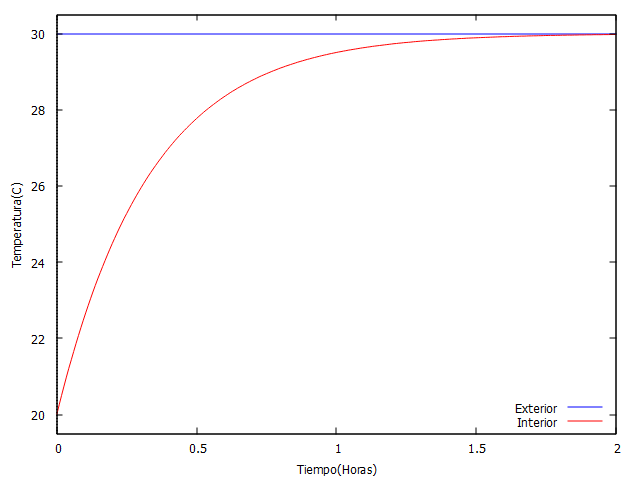
\includegraphics[width=0.7\textwidth]{grafica_ej1_tempconstante}
		\caption{Variación de la temperatura manteniendo la temperatura exterior constante}
		\label{fig:constante1}
	\end{figure}
\end{ejemplo}

\begin{ejemplo}
	Determinar la temperatura del edificio $T(t)$ si la razón de calentamiento adicional $H(t)$ es igual a la constante $H_0$, no hay calentamiento ni enfriamiento $(U(t) = 0)$ y la temperatura exterior $M$ varía como una onda senoidal en un periodo de 24 horas, con un mínimo en $t = 0$ (medianoche) y un máximo en $t = 12$ (mediodía). Es decir, 
	\begin{equation}
		M(t) = M_0 - B \cos \omega t,
	\end{equation}
	donde $B$ es una constante positiva, $M_0$ es la temperatura exterior promedio y $\omega = 2\pi /24 =\pi /12$ radianes/hora. (Esto podría ocurrir durante la primavera o el otoño cuando no hay calefactor ni aire acondicionado).\\
	\textbf{Solución.} La función $Q(t)$ que vimos en~\eqref{eq:apli1} ahora es
	\begin{equation}
		Q(t) = K(M_0 - B \cos \omega t) + H_0.
	\end{equation}
	Al hacer $B_0 := M_0 + H_0/K$, podemos escribir $Q$ como
	\begin{equation}
		Q(t) = K(B_0 - B \cos \omega t),
	\end{equation}
	donde $KB_0$ representa el valor promedio diario de $Q(t)$, es decir,
	\begin{equation}
		KB_0 = \dfrac{1}{24}\int_{0}^{24}Q(t)dt.
	\end{equation}
	Cuando la función de forzamiento $Q(t)$ que hemos obtenido se sustituye en la expresión para la temperatura en la ecuación~\eqref{eq:apli2}, el resultado, después de integrar por partes, es
	\begin{equation}
		T(t) = e^{-Kt}[\int e^{Kt}(KB_0 - KB \cos \omega t)dt + C]
	\end{equation}
	\begin{equation}\label{eq:apli3}
		T(t) = B_0 - BF(t) + Ce^{-Kt},
	\end{equation}
	donde
	\begin{equation}
		F(t) := \dfrac{\cos \omega t + (\omega / K) \sin \omega t}{1 + (\omega /K)^2}
	\end{equation}
	Elegimos la constante $C$ de modo que en medianoche $(t=0)$, el valor de temperatura $T$ sea igual a cierta temperatura inicial $T_0$. Así,
	\begin{equation}
		C = T_0 - B_0 + BF(0) = T_0 - B_0 + \dfrac{B}{1 + (\omega /K)^2}.
	\end{equation}
	Observamos que el tercer término de la solución~\eqref{eq:apli3} que multiplica a la constante $C$ tiende a cero exponencialmente. El término constante $B_0$ es igual a $M_0 + H_0/K$y representa la temperatura promedio diaria dentro del edificio (despreciando el término exponencial). Cuando no hay una razón de calentamiento adicional dentro del edificio $(H_0 = 0)$, esta temperatura promedio es igual a la temperatura exterior promedio $M_0$. El término $BF(t)$ representa la variación senoidal de la temperatura dentro del edificio correspondiente a la variación de la temperatura en el exterior.
	
	Como $F(t)$ se puede escribir en la forma
	\begin{equation}
		F(t) = [1 + (\omega /K)^2]^{-1/2}\cos (\omega t - \phi),
	\end{equation}
	donde $\tan \phi = \omega /K$, la variación senoidal dentro del edificio se retrasa con respecto de la variación en el exterior por $\phi / \omega$ horas. Además, la magnitud de la variación dentro del edificio es ligeramente menor, por un factor de $[1 + (\omega /K)^2]^{-1/2}$, que la variación en el exterior. La frecuencia angular de variación $\omega$ es $2 \pi / 24$ radianes/hora (aproximadamente $1/4$). Los valores usuales para la razón adimensional $\omega /K$ están entre $1/2$ y $1$. Para este rango, el retraso entre la temperatura interior y la exterior es aproximadamente de $1.8$ a $3$ horas y la magnitud de la variación interior está entre $89$ y $71\%$ de la variación en el exterior.
	\begin{figure}[h!]
		\centering
		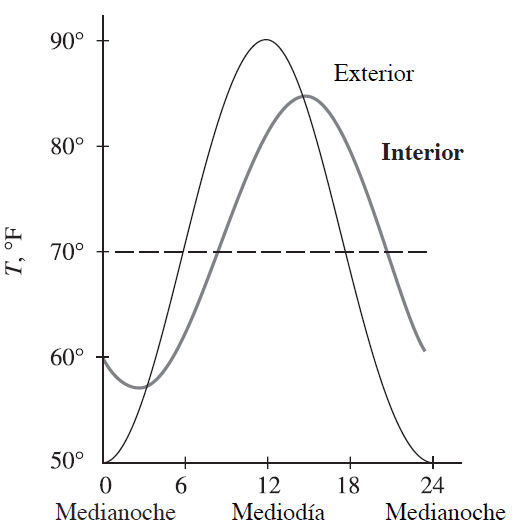
\includegraphics[width=0.7\textwidth]{fig_aplicacion1}
		\caption{Variación de la temperatura dentro y fuera de un edificio sin calefacción}
		\label{fig:aplicacion1}
	\end{figure}
	En la \autoref{fig:aplicacion1} podemos ver la variación senoidal de 24 horas de la temperatura exterior para un día moderado típico así como las variaciones de temperatura dentro del edificio para una razón adimensional $\omega /K$ de la unidad, que corresponde a una constante de tiempo $1/K$ de aproximadamente 4 horas. Los valores que hemos tomado para realizar este ejemplo concreto son:
	\begin{itemize}
		\item $M_0 = 10\celsius$ (Temperatura exterior promedio)
		\item $T_0 = 10\celsius$ (Temperatura interior inicial)
		\item $K = 0.4$
		\item $B = 4$
	\end{itemize}
	Podemos ver cómo la temperatura interior del edificio sigue el comportamiento esperado, es decir, disminuye cuando es mayor que la exterior, y viceversa, y además, a mayor es la distancia entre ambas temperaturas, mayor es la variación de la temperatura interior del edificio, como es natural.
	Al trazar esta última curva, hemos supuesto que el término exponencial ha desaparecido.
\end{ejemplo}
\section{Ejemplo con dos habitaciones}
Ahora consideremos el mismo problema con dos zonas, de modo que el calor se transfiere de una a otra en función de la diferencia de temperatura. Suponemos además que alguna de las zonas posee una fuente de calor (o de enfriamiento) que hará que ésta se caliente (o enfríe) en función de su capacidad calorífica. La variación de temperatura en cada zona será la suma del calor (o frío) generado por dicha fuente, si existe en esa zona, y la pérdida o ganancia de calor generada por el contacto con otras zonas o con el exterior. Para calcular las ecuaciones aplicaremos la \textit{ley de Newton del enfriamiento} vista anteriormente.
\begin{ejemplo}
	Un estudio consta de dos zonas: la zona A de la planta alta y la zona B de la planta baja como podemos ver en la \autoref{fig:aplicacion2}. La planta baja, que tiene una capacidad calorífica de $(1/5)\degree C /1000$ btu (btu: unidades térmicas británicas), es calentada por un calefactor que genera $90000$ btu por hora. Las constantes de tiempo de transferencia de calor son: $3$ horas entre la planta baja y el exterior, $1/2$ hora entre la planta alta y el exterior y $1/2$ hora entre las dos plantas. Si la temperatura en el exterior permanece constante a $2\degree C$ e inicialmente ambas zonas estaban a $22\degree C$, calculemos la temperatura en la planta baja al cabo de $1$ hora.
	
	\begin{figure}[h!]
		\centering
		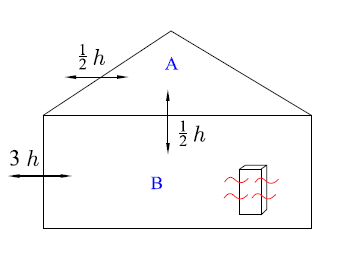
\includegraphics[width=0.6\textwidth]{aplicacion2}
		\caption{Calentamiento de edificio compuesto por dos zonas.}
		\label{fig:aplicacion2}
	\end{figure}
	\textbf{Solución.} En este caso, tenemos tres regiones, la zona A, la zona B y el exterior, luego tendremos que tener en cuenta la transferencia de calor entre
	las tres.
	
	Sea $x(t)$ la temperatura en la zona $A$ en un instante $t$ y sea $y(t)$ la temperatura en la zona $B$ en un instante $t$.
	
	La zona B recibe el calor generado por el calefactor a razón de $90000 btu/h$, puesto que su capacidad calorífica es de  $(1/5)\degree C /1000$ btu, tendremos que la temperatura que gana $B$ es:
	\begin{equation}
		90000 btu/h \times (1/5)\degree C /1000 btu = 18\degree C/h.
	\end{equation}
	La variación de temperatura en las zonas $A$ y $B$ vendrá dada por:
	\begin{equation}
		\dfrac{dx}{dt} = 2(2-x)+2(y-x)
	\end{equation}
	\begin{equation}
		\dfrac{dy}{dt} = \dfrac{1}{3}(2-y)+2(x-y) + 18.
	\end{equation}
	Por tanto, tenemos el sistema no homogéneo:
		\begin{equation}
		\dfrac{dx}{dt} = -4x+2y-4
	\end{equation}
	\begin{equation}
		\dfrac{dy}{dt} = 2x-\dfrac{7}{3}y+\dfrac{56}{3}
	\end{equation}
	Resolvamos el sistema. La ecuación característica es:
	\begin{equation}
		\begin{vmatrix} -4-r & 2 \\ 2 & -\dfrac{7}{3}-r \end{vmatrix} = 0 \rightarrow 3r^2 + 19r + 16 =0,
	\end{equation}
	cuyas raíces son los valores propios: $r_1 = -1 y r_2 = -\dfrac{16}{3}$. Calculemos los vectores propios asociados a cada valor:
	\begin{equation}
		H_{-1} = \{(x,y): \begin{pmatrix}
			-3 & 2\\ 
			2 & -\dfrac{4}{3} 
		\end{pmatrix} \begin{pmatrix}
		x \\ 
		y
		\end{pmatrix} = \begin{pmatrix}
		0 \\ 
		0  
		\end{pmatrix}\} = \{(x,y): -3x + 2y = 0\},
	\end{equation}
	\begin{equation}
		H_{-16/3} = \{(x,y): \begin{pmatrix}
			\dfrac{4}{3} & 2\\ 
			2 & 3
		\end{pmatrix} \begin{pmatrix}
			x \\ 
			y
		\end{pmatrix} = \begin{pmatrix}
			0 \\ 
			0  
		\end{pmatrix}\} = \{(x,y): 2x + 3y = 0\},
	\end{equation}
	Por tanto, un vector propio asociado a $r_1 = -1$ es $\vec{u}_1 = \begin{pmatrix}
		2 \\ 
		3
	\end{pmatrix}$ y un vector propio asociado a $r_2 = -\dfrac{16}{3}$ es $\vec{u}_2 = \begin{pmatrix}
	3 \\ 
	-2
	\end{pmatrix}$ y la solución de la parte homogénea resulta:
	\begin{equation}
		\vec{x}_h(t) = \begin{pmatrix}	x_h(t) \\ y_h(t)	\end{pmatrix} = C_1e^{-t}\begin{pmatrix}	2 \\ 3	\end{pmatrix} + C_2e^{-16t/3}\begin{pmatrix}	3 \\ -2	\end{pmatrix}.
	\end{equation}
	Ahora buscamos una solución particular mediante el método de los coeficientes
	indeterminados. Puesto que el término no homogéneo es un polinomio de grado
	$0$ y además $0$ no es raíz de la ecuación característica, podemos tomar la solución particular de la forma:
	\begin{equation}
		\vec{x}_p = \vec{a} = \begin{pmatrix}	a_1 \\ a_2	\end{pmatrix}.
	\end{equation}
	Derivando y sustituyendo en la ecuación, tenemos:
	\begin{equation}
		\begin{pmatrix}	0 \\ 0	\end{pmatrix} = \begin{pmatrix}
		    -4 & 2\\ 
			2 & -\dfrac{7}{3}
		\end{pmatrix} \begin{pmatrix}	a_1 \\ a_2	\end{pmatrix} +  \begin{pmatrix}	4 \\ 56/3	\end{pmatrix}
	\end{equation}
	pasando el término independiente al otro lado de la igualdad,
	\begin{equation}
		\begin{pmatrix}
			-4 & 2\\ 
			2 & -\dfrac{7}{3}
		\end{pmatrix}\begin{pmatrix}	a_1 \\ a_2	\end{pmatrix} = \begin{pmatrix}	-4 \\ -	56/3\end{pmatrix}
	\end{equation}
	de donde obtenemos: $a_1 = 35/4$ y $a_2 = 31/2.$ La solución general es:
	\begin{equation}
		\vec{x}(t) = \begin{pmatrix}	x(t) \\ y(t)	\end{pmatrix} = C_1e^{-t}\begin{pmatrix}	2 \\ 3	\end{pmatrix} + C_2e^{-16t/3}\begin{pmatrix}	3 \\ -2	\end{pmatrix} + \begin{pmatrix}	35/4 \\ 31/2	\end{pmatrix}
	\end{equation}
	Considerando las condiciones iniciales: para $t=0, x(0) = 22$ y $y(0) = 22$, se tiene:
	\begin{equation}
		\begin{pmatrix}	22 \\ 22	\end{pmatrix} = C_1 \begin{pmatrix}	2 \\ 3	\end{pmatrix} + C_2 \begin{pmatrix}	3 \\ -2	\end{pmatrix} + \begin{pmatrix}	35/4 \\ 31/2	\end{pmatrix}
	\end{equation}
	Agrupando los términos independientes y reescribiendo los sumandos multiplicados
	por las constantes $C_1$ y $C_2$ en términos de la matriz fundamental, tenemos:
	\begin{equation}
		\begin{pmatrix}
			2 & 3\\ 
			3 & -2
		\end{pmatrix}\begin{pmatrix}	C_1 \\ C_2	\end{pmatrix} = \begin{pmatrix}	53/4 \\ 13/2	\end{pmatrix}
	\end{equation}
	y resolviendo el sistema obtenemos:
	\begin{equation}
		C_1 = 46/13 \qquad y \qquad C_2 = 107/52.
	\end{equation}
	La solución a este problema de valor inicial es:
	\begin{equation}
		\vec{x}(t) = \begin{pmatrix}	x(t) \\ y(t)	\end{pmatrix} = \dfrac{46}{13}e^{-t}\begin{pmatrix}	2 \\ 3	\end{pmatrix} + \dfrac{107}{52}e^{-16t/3}\begin{pmatrix}	3 \\ -2	\end{pmatrix} + \begin{pmatrix}	35/4 \\ 31/2	\end{pmatrix}.
	\end{equation}
	Puesto que la temperatura en $B$ era $y(t)$, ésta al cabo de $1h$ será:
	\begin{equation}
		y(1) = \dfrac{46}{13}e^{-t}3 + \dfrac{107}{52}e^{-16t/3}(-2) + \dfrac{31}{2} \approx 19,405\degree C.
	\end{equation}
\end{ejemplo}

\section{Modelos de un edificio con 5 habitaciones}
\subsection{Primer ejemplo (temperatura exterior constante)}
Vamos a estudiar un par de casos de edificios con 5 habitaciones, donde incluiremos personas, y aires acondicionados para hacer el edificio más realista. El primer caso será el que tenemos en la \autoref{fig:edif5}. Podemos ver $5$ habitaciones contiguas y $2$ aires acondicionados en las habitaciones $B$ y $D$. Los datos que tomaremos son los siguientes:
\begin{itemize}
	\item Temperatura en A $\rightarrow a(t)  $ 
	\item Temperatura en B $\rightarrow b(t)  $ 
	\item Temperatura en C $\rightarrow c(t)  $ 
	\item Temperatura en D $\rightarrow d(t)  $ 
	\item Temperatura en E $\rightarrow e(t)  $ 
	\item Temperatura en el exterior F $\rightarrow M(t) = 35 \celsius$ 
	\item Constante de transferencia entre cada habitación $K = 2$
	\item Constante de transferencia entre una habitación y el exterior $K_{xF} = 4$
	\item Calor generado por cada aire acondicionado U $\rightarrow U(t) = -4\celsius / 5h$
	\item Calor generado en el interior H $\rightarrow H(t) = 0$
\end{itemize}
\begin{figure}[h!]
	\centering
	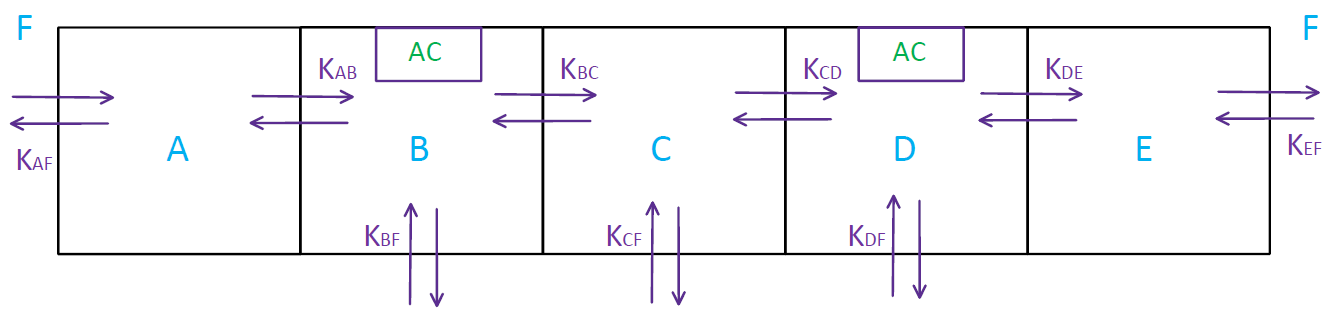
\includegraphics[width=\textwidth]{edificio_5habs}
	\caption{Edificio con 5 habitaciones contiguas}
	\label{fig:edif5}
\end{figure}
Observando la estructura del edificio, obtenemos el siguiente sistema de ecuaciones:
\begin{equation}\begin{dcases}
	 a'(t)= \dfrac{b(t)-a(t)}{K_{AB}} + \dfrac{M(t) - a(t)}{K_{AF}} \\  b'(t)= \dfrac{a(t)-b(t)}{K_{AB}} + \dfrac{c(t)-b(t)}{K_{BC}} + \dfrac{M(t) - b(t)}{K_{BF}} + U_B(t) \\ c'(t)= \dfrac{b(t)-c(t)}{K_{BC}} + \dfrac{d(t)-c(t)}{K_{CD}} + \dfrac{M(t) - c(t)}{K_{CF}} \\  d'(t)= \dfrac{c(t)-d(t)}{K_{CD}} + \dfrac{e(t)-d(t)}{K_{DE}} + \dfrac{M(t) - d(t)}{K_{DF}} + U_D(t) \\  e'(t)= \dfrac{d(t)-e(t)}{K_{DE}} + \dfrac{M(t) - e(t)}{K_{EF}} \end{dcases}
\end{equation}
Como valores iniciales para las temperaturas de cada habitación tomaremos:
\begin{equation}
	a(t_0) = 25 \celsius, \qquad b(t_0) = 25 \celsius, \qquad c(t_0) = 28 \celsius, \qquad d(t_0) = 20 \celsius, \qquad e(t_0) = 20 \celsius.
\end{equation}
Resolvemos el sistema con $Maxima$ y obtenemos la solución gráficamente en la \autoref{fig:graf_sol1}.
\begin{figure}[h!]
	\centering
	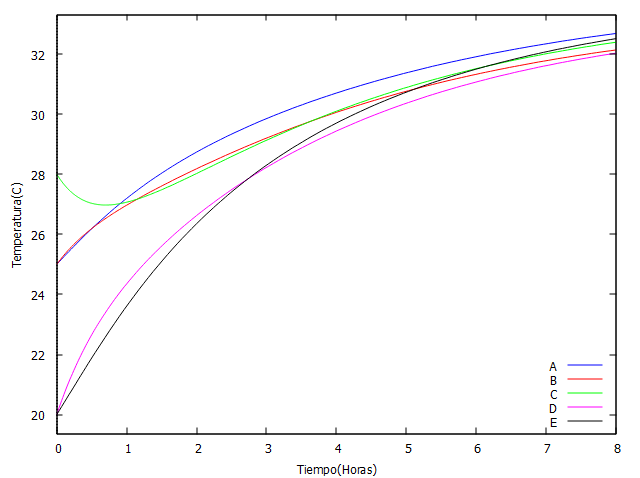
\includegraphics[width=\textwidth]{graf_sol_5habs1}
	\caption{Temperaturas de las 5 habitaciones con temperatura exterior constante de $35 \celsius$}
	\label{fig:graf_sol1}
\end{figure}
Es importante observar varias cosas:
\begin{itemize}
	\item Las habitaciones $D$ y $E$ comienzan con la misma temperatura, pero hasta la tercera hora hace más calor en la habitación $D$, ¿Cómo puede ser si esta habitación tiene aire acondicionado? Pues porque está pegada a la habitación $C$ en la que hace mucho más calor, luego la variación de temperatura se ve más afectada por esto que por el aire acondicionado, pero vemos como cuando todas las habitaciones se van aproximando en cuanto a temperatura, el efecto del aire acondicionado hace que la habitación $D$ sea la más fresquita, como era de esperar.
	\item Por un motivo similar, vemos que la habitación $C$ incluso se enfría en la primera hora, pese a que fuera están a $35 \celsius$, esto es debido a que la constante de transferencia $K$ entre cada habitación es menor que hacia el exterior, y al estar las otras habitaciones más frías al principio, se enfría un poco, pero en cuanto todas las demás habitaciones se van calentando, deja de tener efecto sobre la habitación $C$ y emprende su camino hacia los $35 \celsius$ del exterior.
	\item Como era de esperar, al principio la variación de temperatura es mayor por haber más diferencia entre las habitaciones y el exterior, y conforme va pasando el tiempo, se van aproximando a los $35 \celsius$ y la variación va disminuyendo.
	\item En general, las habitaciones $A$ y $E$ son las que más variación de temperatura tienen, esto es naturalmente debido a que sólo tienen cerca una habitación, y se ven más influenciadas por el exterior, además de que no tienen aire acondicionado.
\end{itemize}
\subsection{Segundo ejemplo (temperatura exterior variable)}
En el siguiente caso vamos a colocar algunas personas en las habitaciones, y además vamos a cambiar un poco la estructura interna del edificio, tomaremos la \autoref{fig:edif5_2} como referencia.

Vamos a tomar como variables:
\begin{itemize}
	\item Temperatura en el exterior F $\rightarrow M(t) = 18-12\cos(t\cdot(\pi/12))$
	\item Constante de transferencia entre cada habitación $K = 2$
	\item Constante de transferencia entre una habitación y el exterior $K_{xF} = 4$
	\item Calor generado por cada aire acondicionado U $\rightarrow U(t) = -2\celsius / h$
	\item Calor generado en el interior H $\rightarrow H(t) = 0.018$ por cada persona
\end{itemize}
\begin{figure}[h!]
	\centering
	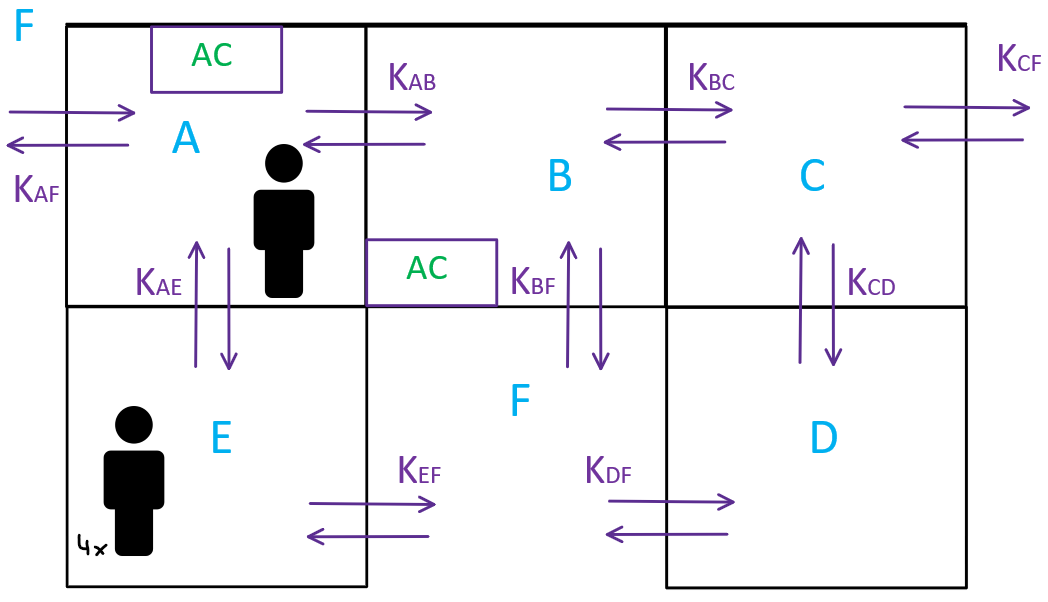
\includegraphics[width=0.8\textwidth]{edificio_5habs2}
	\caption{Edificio con 5 habitaciones, 1 persona en A y 4 personas en E}
	\label{fig:edif5_2}
\end{figure}
Atendiendo a la estructura del edificio, obtenemos el siguiente sistema:
\begin{equation}\begin{dcases}
		a'(t)= \dfrac{b(t)-a(t)}{K_{AB}} + \dfrac{e(t)-a(t)}{K_{AE}} + \dfrac{M(t) - a(t)}{K_{AF}} + U_A(t) + H(t) \\  b'(t)= \dfrac{a(t)-b(t)}{K_{AB}} + \dfrac{c(t)-b(t)}{K_{BC}} + \dfrac{M(t) - b(t)}{K_{BF}} + U_B(t) \\ c'(t)= \dfrac{b(t)-c(t)}{K_{BC}} + \dfrac{d(t)-c(t)}{K_{BC}} + \dfrac{M(t) - c(t)}{K_{CF}} \\  d'(t)= \dfrac{c(t)-d(t)}{K_{BD}} + \dfrac{M(t) - d(t)}{K_{DF}} \\  e'(t)= \dfrac{a(t)-e(t)}{K_{AE}} + \dfrac{M(t) - e(t)}{K_{EF}} + 4H(t) \end{dcases}
\end{equation}
Como valores iniciales para las temperaturas de cada habitación tomaremos:
\begin{equation}
	a(t_0) = 10 \celsius, \qquad b(t_0) = 0 \celsius, \qquad c(t_0) = 12 \celsius, \qquad d(t_0) = 17 \celsius, \qquad e(t_0) = 8 \celsius.
\end{equation}
Ahora resolvemos el sistema con $Maxima$ y obtenemos las temperaturas de cada habitación gráficamente en la \autoref{fig:graf_sol2}.
\begin{figure}[h!]
	\centering
	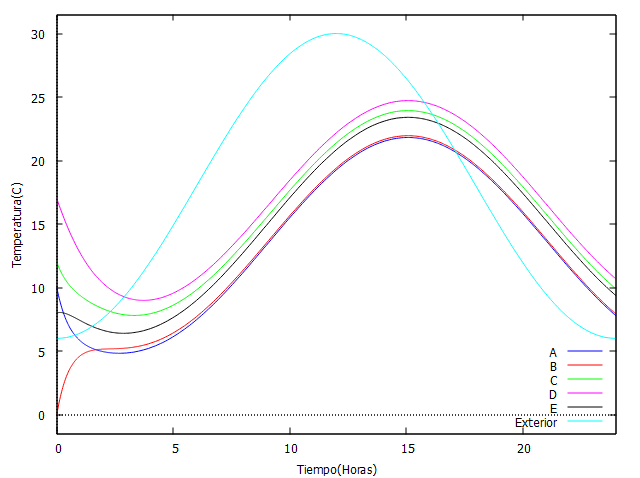
\includegraphics[width=\textwidth]{graf_sol_5habs2}
	\caption{Temperaturas de las 5 habitaciones con temperatura exterior variable}
	\label{fig:graf_sol2}
\end{figure}
En este caso tenemos varios detalles que observar:
\begin{itemize}
	\item Se aprecia perfectamente cómo la temperatura interior tiene una variación más suave que la exterior, algo natural debido a los aislantes térmicos que tiene el edificio.
	\item Vemos cómo las habitaciones $A$ y $B$, que tienen un potente aire acondicionado, siempre se mantienen más frías que el resto durante todo el día.
	\item Pese a que al principio cada habitación tiene una temperatura bastante diferente, al final todas se van aproximando entre ellas, debido a que lo que más las influencia es la temperatura exterior, es decir, es el mayor factor que afecta a la variación de su temperatura.
\end{itemize}
\endinput
%------------------------------------------------------------------------------------
% FIN DEL CAPÍTULO. 
%----------------------------------------------------------------------------------
-